\documentclass{article}
\usepackage[letterpaper,top=2cm,bottom=2cm,left=3cm,right=3cm,marginparwidth=1.75cm]{geometry}
\usepackage{tikz}
\usetikzlibrary{automata, arrows.meta, positioning}
\usepackage{amsmath}
\usepackage{graphicx}
\usepackage[colorlinks=true, allcolors=blue]{hyperref}
\usepackage[spanish]{babel}
\usepackage[style=apa]{biblatex}
 \usepackage{listings}


\begin{document}
\begin{titlepage}
\centering
\begin{figure}
\centering
 
\vspace{5cm}
\centering
\begin{Huge}
\begin{center}


\includegraphics[scale=0.2]{imagenes/logo.png} 

\vspace{1cm}
\end{center}

\end{Huge}
\end{figure}


 {\scshape\Large Práctica creación de paquetes\par}
\vspace{9cm}

{\Large Ignacio Fernández Contreras\par}
{\Large 4º Informática A\par}
\vspace{0.5cm}
{\large E.T.S. Informática}
\vfill

\end{titlepage}
\clearpage\hbox{}\thispagestyle{empty}\newpage

%-------------------------- EJERCICIO 1 ----------------------

 \newpage
\section{Enunciado}
\begin{flushleft}
El objetivo de la práctica es automatizar la instalación de una aplicación de usuario mediante
la creación de un paquete para el sistema operativo Ubuntu Server. Para ello se pide:
\begin{enumerate}
\item Crear una aplicación que será empaquetada en formato Debian binario .deb. La
aplicación deberá realizar una lógica a elegir por el usuario, y deberá contar con una
dependencia de otro paquete (e.g. hwinfo) que será invocada en la lógica desarrollada
(mirar función popen), por ejemplo, para imprimir el resultado por pantalla, y deberá
ser instalada en el sistema.
\item  Una vez instalado el paquete se debe comprobar que se ha instalado el mismo y la
dependencia utilizada
\item  Describir de forma detallada los pasos realizados para empaquetar dicha aplicación, la
estructura de archivos y las instrucciones necesarias para instalarla adecuadamente.
\end{enumerate}
Nota: para instalar dependencias después de instalar el paquete con dpkg-deb se puede utilizar sudo apt-get -f install
OPCIONAL: Describir el proceso a través del cual se puede crear un repositorio PPA de
Ubuntu donde poder alojar y distribuir una versión fuente del paquete creado
\end{flushleft}

 \section{Resolución}
 
Vamos a empezar creando el arbol completo de myapp, para ello vamos a utilizar el comando 

  \lstset{language=C, breaklines=true, basicstyle=\footnotesize}
\begin{lstlisting}[frame=single]
mkdir myapp
cd myapp/
mkdir DEBIAN
mkdir usr/bin
\end{lstlisting}

Obteniendo así, el siguiente árbol:
\begin{center}
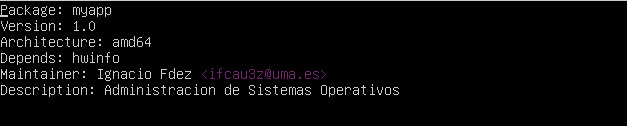
\includegraphics[scale=0.6]{imagenes/im1.png} 
\end{center}
Creamos ahora el fichero de control:
\begin{center}
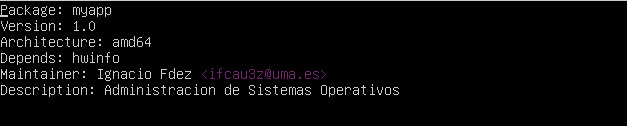
\includegraphics[scale=0.6]{imagenes/img2.png} 
\end{center}
Como se puede ver, en el fichero de control tiene añadida una dependencia a hwinfo.\\
El fichero myapp.sh quedaría:
  \lstset{language=C, breaklines=true, basicstyle=\footnotesize}
\begin{lstlisting}[frame=single]
#!/bin/bash
echo "Hola!"
\end{lstlisting}

Una vez creado ambos ficheros, empaquetamos el paquete:

  \lstset{language=C, breaklines=true, basicstyle=\footnotesize}
\begin{lstlisting}[frame=single]
dpkg-deb --build myapp
\end{lstlisting}

y obtenemos un fichero "myapp.deb"\\
Para instalar y ejercutar el programa:

  \lstset{language=C, breaklines=true, basicstyle=\footnotesize}
\begin{lstlisting}[frame=single]
sudo dpkg -i myapp.deb
myapp.sh
\end{lstlisting}
\begin{center}
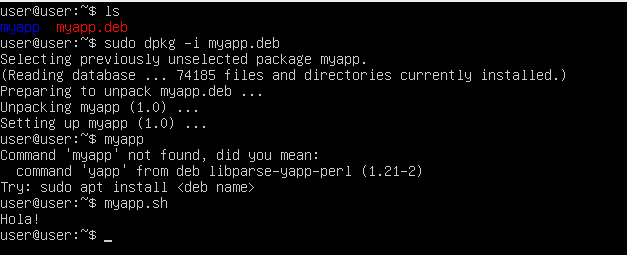
\includegraphics[scale=0.6]{imagenes/img3.png} 
\end{center}


\textbf{Describir el proceso a través del cual se puede crear un repositorio PPA de Ubuntu donde poder alojar y distribuir una versión fuente del paquete creado.}

Preparamos el entorno:

  \lstset{language=C, breaklines=true, basicstyle=\footnotesize}
\begin{lstlisting}[frame=single]
sudo apt install dput
\end{lstlisting}
dput es la herramienta que utilizaremos para subir los paquetes al PPA (\textit{Personal Package Archive})

Configuramos el entorno:


  \lstset{language=C, breaklines=true, basicstyle=\footnotesize}
\begin{lstlisting}[frame=single]
gpg --gen-key
\end{lstlisting}
Esto nos dará paso a configurar una clave
\begin{center}
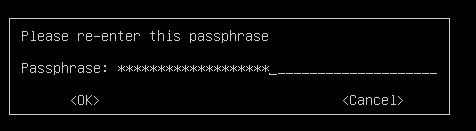
\includegraphics[scale=0.6]{imagenes/img4.png} 
\end{center}
Creando (RSA) y firmando la clave pública y privada
\begin{center}
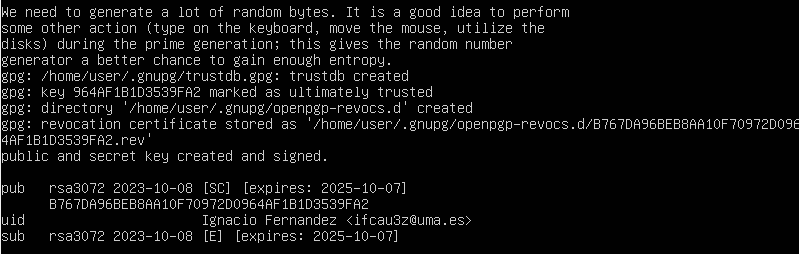
\includegraphics[scale= 0.6]{imagenes/img5.png} 
\end{center}

Creamos el archivo fuente .dsc:


\lstset{language=C, breaklines=true, basicstyle=\footnotesize}
\begin{lstlisting}[frame=single]
debuild -S -sa
\end{lstlisting}
\newpage
Ahora, hay que crear un par de archivos adicionales, que para la creación del paquete de ejemplo no fueron necesarios:
\begin{itemize}
\item Fuente
\end{itemize}

\lstset{language=C, breaklines=true, basicstyle=\footnotesize}
\begin{lstlisting}[frame=single]
myapp (1.0-1) unstable; urgency=low
	*Initial release
	-- Ignacio Fdez <ifcau3z@uma.es> Sund, 08 Oct
\end{lstlisting}


\begin{itemize}
\item Rules
\end{itemize}

\lstset{language=C, breaklines=true, basicstyle=\footnotesize}
\begin{lstlisting}[frame=single]
#!/usr/bin/make -f
%:
	dh $@
\end{lstlisting}


Quedando el paquete con la siguiente forma:
\begin{center}
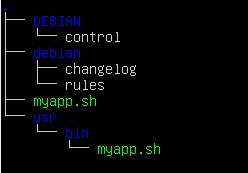
\includegraphics[scale=1]{imagenes/img6.png} 
\end{center}


Una vez creado el fichero .dsc, para subirlo a PPA:

\lstset{language=C, breaklines=true, basicstyle=\footnotesize}
\begin{lstlisting}[frame=single]
dput ppa: ppa_username/myapp mypackage_version_source.changes
\end{lstlisting}




\end{document}